% --- RAPPORT ---
\newpage
\section*{Introduction}
\addcontentsline{toc}{section}{Introduction}

\subsection*{Présentation du projet}
\phantomsection
\addcontentsline{toc}{subsection}{Présentation du projet}

Le présent rapport expose la stratégie de modernisation et de sécurisation du Système d’Information (SI) de l’entreprise XANADU. À l’occasion de son déménagement vers la technopole Atlantis et de l'ouverture d'un nouveau bureau à Springfield, XANADU souhaite transformer son infrastructure actuelle pour la rendre plus robuste.

\subsection*{Contexte et enjeux}
\phantomsection
\addcontentsline{toc}{subsection}{Contexte et enjeux}

\noindent Actuellement, l’entreprise fait face à des défis majeurs :

\begin{itemize}
    \item Sécurité accrue : Suite aux récentes cyberattaques par rançongiciel (ransomware) subies par des partenaires, la direction exige un système capable de résister aux menaces et de garantir la protection des données.
    \item Continuité d'activité : L'objectif est de garantir une reprise de service sous 4 heures pour les outils critiques (comme l'ERP) et 24 heures pour les autres services.
    \item Centralisation des données : Le passage d'une gestion locale (clés USB, dossiers sur PC) à une gestion centralisée est nécessaire pour assurer la cohérence et la sauvegarde des documents de travail.
\end{itemize}

\subsection*{Objectifs de la mission}
\phantomsection
\addcontentsline{toc}{subsection}{Objectifs de la mission}

\noindent La mission confiée à notre équipe CESITECH se décline en trois axes principaux :

\begin{itemize}
    \item Fiabilité : Interconnecter de manière stable les sites d'Atlantis et de Springfield via un tunnel sécurisé.
    \item Accessibilité : Permettre le télétravail et l'accès distant pour les commerciaux en toute sécurité.
    \item Confidentialité : Mettre en place une gestion stricte des droits d'accès pour que chaque service (RH, Juridique, Commercial, etc.) ne voie que ce qui le concerne.
\end{itemize}

\newpage

\section*{Présentation globale de l'architecture}
\addcontentsline{toc}{section}{Présentation globale de l'architecture}

\subsection*{Topologie globale}
\phantomsection
\addcontentsline{toc}{subsection}{Topologie globale}

Pour répondre aux besoins de XANADU, nous avons choisi une topologie en étoile. 

\begin{center}
    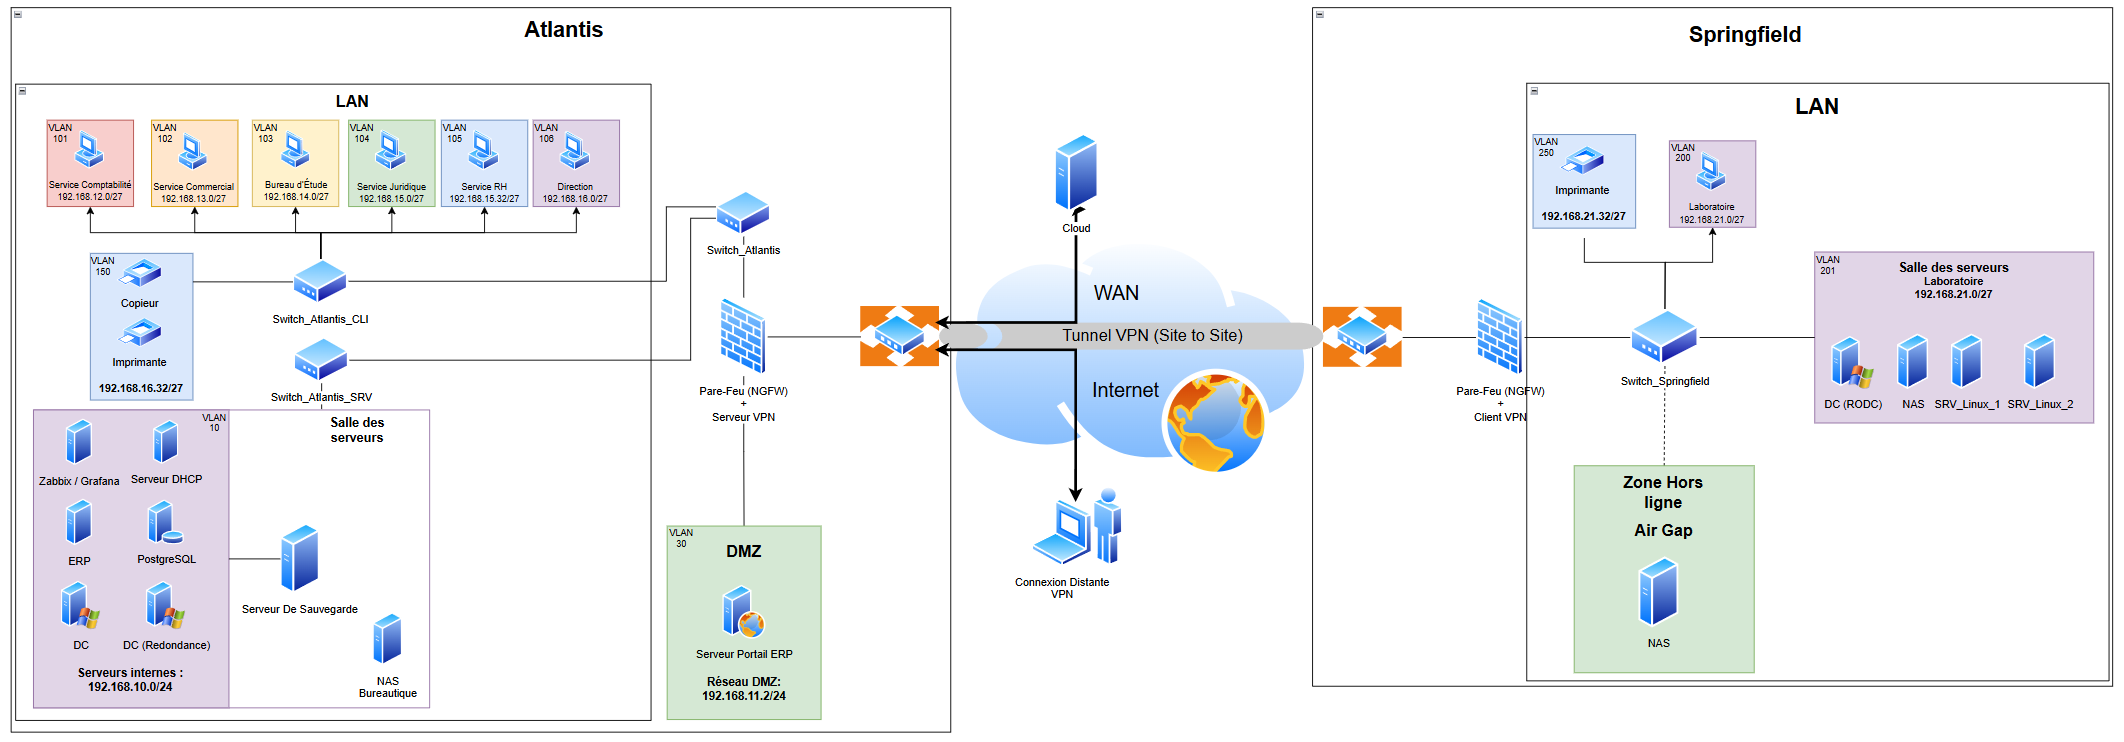
\includegraphics[width=0.9\textwidth]{contents/img/archi_global.png}
\end{center}

Cette structure permet de centraliser les ressources critiques tout en gardant une gestion simplifiée.

\begin{itemize}
    \item Le Cœur du réseau (Site Atlantis) : C'est le site principal. Il héberge la majorité des serveurs (ERP, Base de données, Active Directory principal). C'est ici que sont prises les décisions de sécurité pour l'ensemble de l'entreprise.
    \item L'extension (Site Springfield) : Le laboratoire de Springfield est relié directement au cœur via une liaison sécurisée. Il consomme les ressources du site principal tout en gardant une autonomie pour ses besoins spécifiques (serveurs Linux métiers).
\end{itemize}

\vspace{0.5cm}

\noindent \textbf{Les avantages de ce choix pour XANADU :}
\begin{itemize}
    \item Sécurité simplifiée : Tous les flux passent par des points de contrôle (Pare-feu) bien définis.
    \item Maintenance facilitée : On administre les services importants au même endroit, ce qui fait gagner du temps.
    \item Évolutivité : Si XANADU ouvre un troisième bureau demain, il suffira de le relier au cœur (Atlantis) de la même manière.
\end{itemize}

\subsection*{Description de l'infrastructure physique}
\phantomsection
\addcontentsline{toc}{subsection}{Description de l'infrastructure physique}

\noindent
\begin{minipage}[t]{0.85\textwidth}
    \textbf{Les Pare-feu (NGFW -- Next Generation Firewall)} \\
    Les pare-feu constituent le premier niveau de défense du système d’information. Positionnés à l’entrée de chaque site, ils assurent la protection périmétrique et le contrôle des échanges entre les différentes zones du réseau.
    
    \vspace{0.5cm}

    \begin{itemize}
        \item \textbf{Rôle :} Filtrage des flux entrants et sortants afin de bloquer les accès non autorisés et les comportements suspects.
        \item \textbf{Fonctions avancées :} Inspection applicative, journalisation des connexions et application de politiques de sécurité différenciées.
        \item \textbf{VPN :} Mise en place et gestion du tunnel VPN site-à-site sécurisé entre Atlantis et Springfield.
    \end{itemize}

    \vspace{0.5cm}

\end{minipage}
\begin{minipage}[t]{0.13\textwidth}
    \vspace{0pt}
    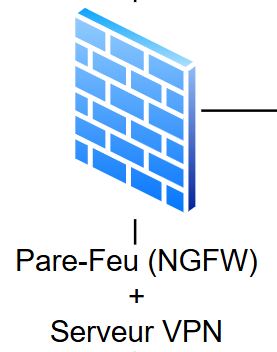
\includegraphics[width=\textwidth]{contents/img/pare-feu.png}
\end{minipage}

\vspace{0.6cm}

\noindent
\begin{minipage}[t]{0.85\textwidth}
    \textbf{Les Routeurs} \\
    Les routeurs assurent l’acheminement du trafic entre les différents réseaux et garantissent la communication entre le LAN interne et les réseaux externes.
    
    \vspace{0.5cm}

    \begin{itemize}
        \item \textbf{Rôle :} Routage des paquets entre les réseaux internes, la DMZ et le WAN.
        \item \textbf{Fonction réseau :} Séparation logique des flux et support de l’architecture multi-sites.
    \end{itemize}

    \vspace{0.5cm}

\end{minipage}
\begin{minipage}[t]{0.12\textwidth}
    \vspace{0pt}
    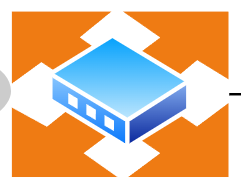
\includegraphics[width=\textwidth]{contents/img/routeur.png}
\end{minipage}

\vspace{0.6cm}

\noindent
\begin{minipage}[t]{0.85\textwidth}
    \textbf{Les Switchs (Commutateurs)} \\
    Les switchs assurent la connectivité interne et la segmentation logique du réseau local.
    \vspace{0.5cm}
    \begin{itemize}
        \item \textbf{Rôle :} Connexion physique des postes de travail, serveurs et périphériques.
        \item \textbf{Segmentation :} Gestion des VLANs permettant de séparer les services (Comptabilité, RH, Direction, etc.).
        \item \textbf{Sécurité :} Réduction des domaines de diffusion et limitation de la propagation des incidents réseau.
    \end{itemize}
\end{minipage}
\begin{minipage}[t]{0.13\textwidth}
    \vspace{0pt}
    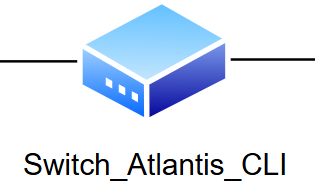
\includegraphics[width=\textwidth]{contents/img/switch.png}
\end{minipage}

\vspace{0.6cm}

\noindent
\begin{minipage}[t]{0.85\textwidth}
    \textbf{Les Serveurs} \\
    Les serveurs constituent le cœur du système d’information de XANADU. Ils hébergent les services critiques indispensables au fonctionnement de l’entreprise et à la continuité de l’activité.
    \vspace{0.5cm}
    \begin{itemize}
        \item \textbf{Services hébergés :} Contrôleurs de domaine Active Directory (authentification, gestion des droits et GPO), ERP, services DNS, DHCP, supervision et sauvegarde.
        \item \textbf{Virtualisation :} Optimisation des ressources matérielles, flexibilité opérationnelle et restauration rapide en cas d’incident.
        \item \textbf{Disponibilité :} Redondance des services critiques afin d’éliminer les points de défaillance uniques.
        \item \textbf{Sécurité :} Intégration dans une architecture segmentée avec filtrage strict des accès.
    \end{itemize}
\end{minipage}
\begin{minipage}[t]{0.10\textwidth}
    \vspace{0pt}
    
\includegraphics[width=\textwidth]{contents/img/serveurs.png}
\end{minipage}

\vspace{0.6cm}

\noindent
\begin{minipage}[t]{0.85\textwidth}
    \textbf{Les Périphériques (Imprimantes et Copieurs)} \\
    Les périphériques représentent des équipements sensibles pouvant constituer des points d’entrée en cas de mauvaise configuration.
    \vspace{0.5cm}
    \begin{itemize}
        \item \textbf{Rôle :} Fournir des services d’impression et de numérisation aux utilisateurs.
        \item \textbf{Sécurité :} Isolation dans un VLAN dédié (VLAN 150) afin d’éviter qu’une compromission ne puisse impacter les serveurs ou le réseau interne.
    \end{itemize}
\end{minipage}
\begin{minipage}[t]{0.11\textwidth}
    \vspace{0pt}
    
\includegraphics[width=\textwidth]{contents/img/imprimante.png}
\end{minipage}

\newpage

\section*{Architecture et Segmentation}
\addcontentsline{toc}{section}{Architecture et Segmentation}

\noindent L’architecture réseau de XANADU repose sur une segmentation logique stricte, combinée à une séparation physique et fonctionnelle des sites. Cette approche vise à garantir un haut niveau de sécurité, de performance et de résilience, tout en assurant la conformité aux bonnes pratiques de l’ANSSI en matière de cloisonnement des zones de confiance.

L’infrastructure est organisée autour de deux sites distincts :
\begin{itemize}
    \item le site principal \textbf{Atlantis}, hébergeant les services critiques et le cœur du système d’information ;
    
    \begin{center}
        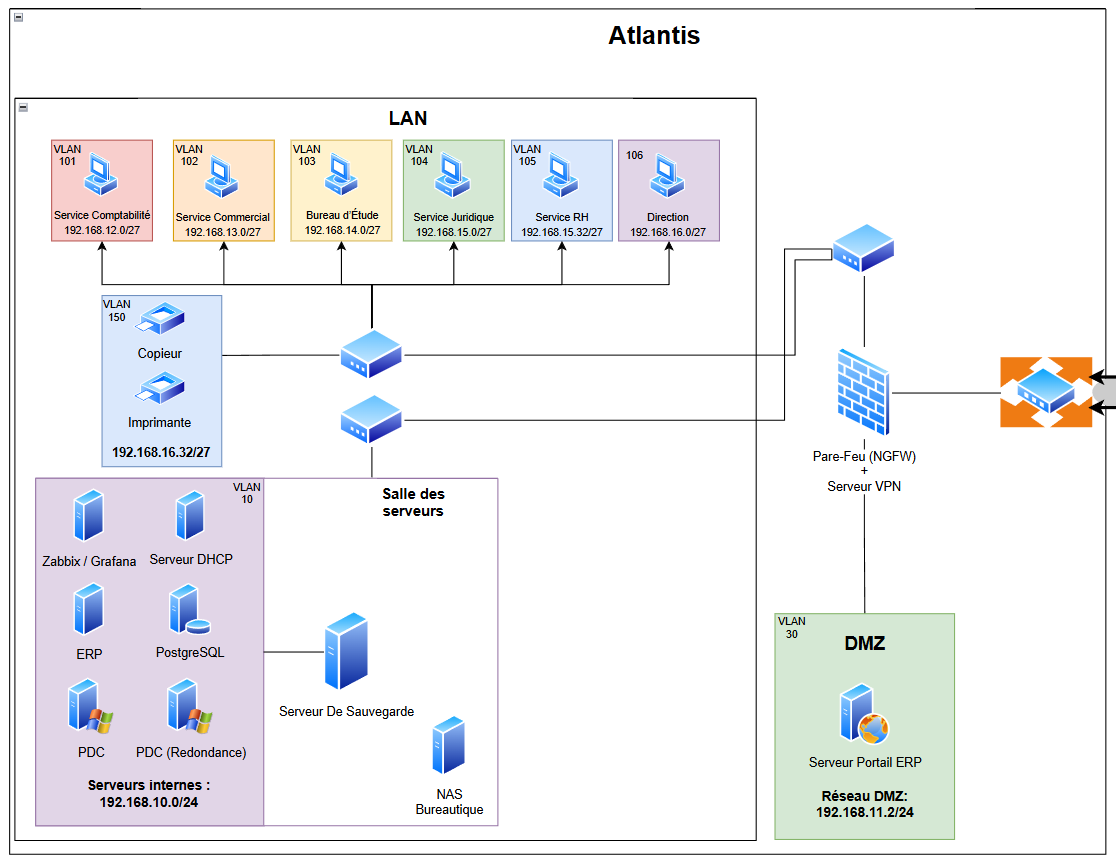
\includegraphics[width=0.5\textwidth]{contents/img/atlantis.png}
    \end{center}

    \item le site distant \textbf{Springfield}, dédié aux activités de laboratoire et disposant d’une autonomie partielle.

    \begin{center}
        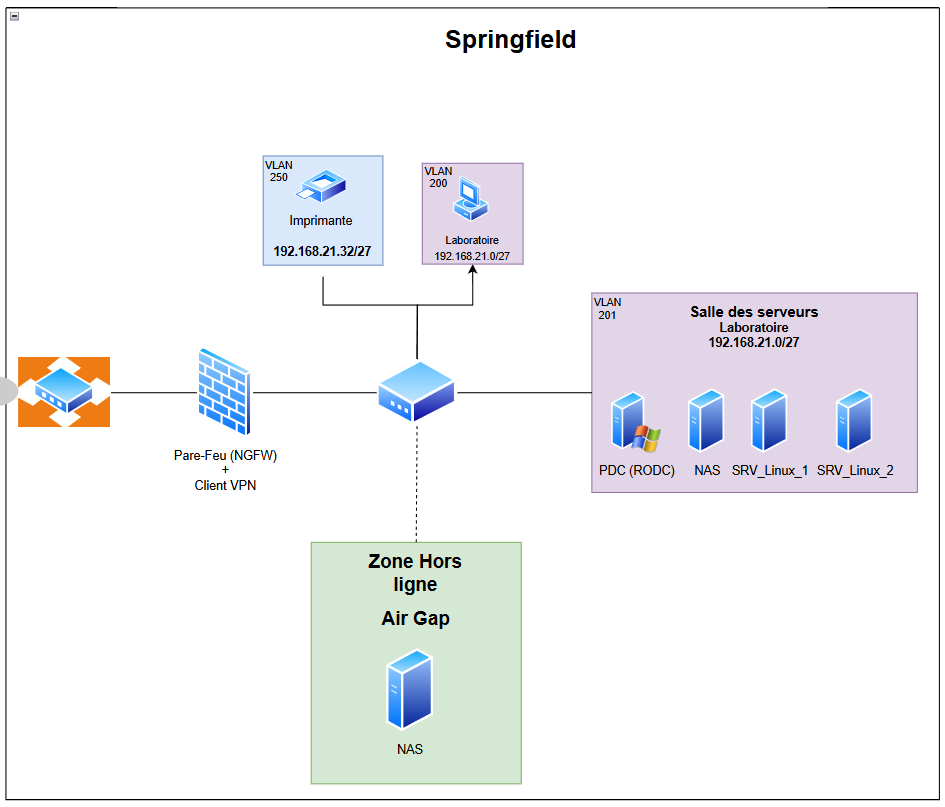
\includegraphics[width=0.5\textwidth]{contents/img/springfield.png}
    \end{center}
\end{itemize}

Ces deux sites sont interconnectés de manière sécurisée via un tunnel VPN site-à-site, assurant la confidentialité, l’intégrité et l’authentification des flux inter-sites.

\subsection*{Sécurité par isolation}
\phantomsection
\addcontentsline{toc}{subsection}{Sécurité par isolation}

La sécurité de l’architecture repose en grande partie sur une stratégie d’isolation stricte des ressources, basée sur le principe de défense en profondeur. Chaque zone fonctionnelle est isolée dans un VLAN dédié, constituant une zone de confiance distincte avec des règles de filtrage spécifiques.

\vspace{0.5cm}

\noindent Sur le site d’Atlantis, le réseau interne est segmenté par service métier :

\begin{center}
        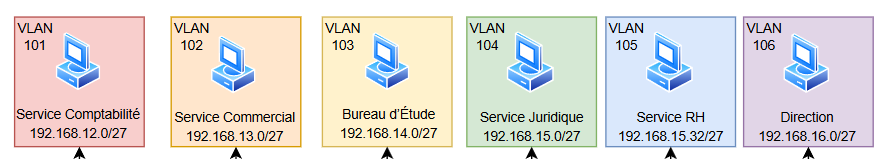
\includegraphics[width=0.8\textwidth]{contents/img/vlan_services.png}
\end{center}

\begin{itemize}
    \item VLAN Service Comptabilité
    \item VLAN Service Commercial
    \item VLAN Bureau d’Études
    \item VLAN Service Juridique
    \item VLAN Ressources Humaines
    \item VLAN Direction
\end{itemize}

\noindent Cette segmentation permet de limiter les déplacements latéraux en cas de compromission d’un poste utilisateur. Un incident affectant un service ne peut ainsi pas se propager librement aux autres services ou aux serveurs critiques.

\vspace{0.5cm}

\noindent \textbf{Les Périphériques (Imprimantes et Copieurs)} \\
Les équipements partagés tels que les imprimantes et copieurs sont placés dans des VLAN dédiés, évitant tout accès direct depuis les postes utilisateurs aux équipements d’infrastructure. Cette isolation réduit considérablement les risques liés aux attaques exploitant des périphériques souvent moins sécurisés.

\begin{itemize}
    \item \textbf{Rôle :} Fournir des services d’impression et de numérisation aux utilisateurs.
    \item \textbf{Sécurité :} Isolation dans un VLAN dédié (VLAN 150) afin d’éviter qu’une compromission ne puisse impacter les serveurs ou le réseau interne.
\end{itemize}

\vspace{0.5cm}
\begin{center}
    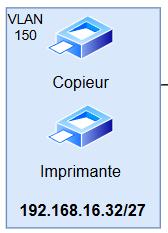
\includegraphics[width=0.2\textwidth]{contents/img/vlan_outils.png}
\end{center}

\noindent Les serveurs internes (ADDS, DNS, DHCP, ERP, PostgreSQL, supervision, sauvegarde) sont regroupés dans un réseau serveurs dédié. 

\vspace{0.5cm}
\begin{center}
    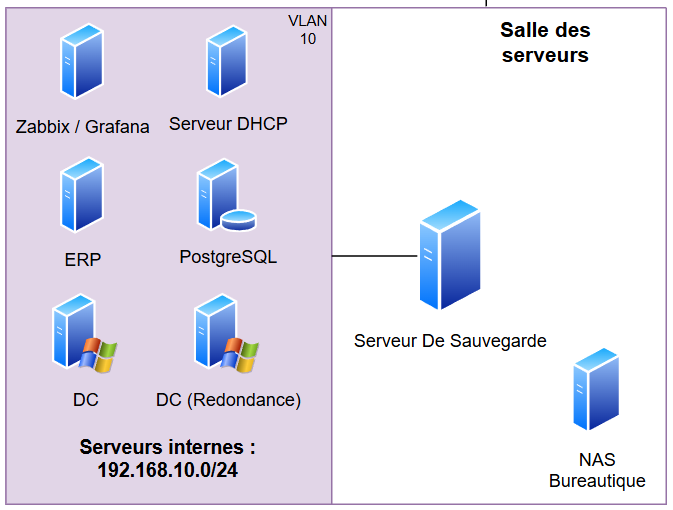
\includegraphics[width=0.6\textwidth]{contents/img/salledesserveurs.png}
\end{center}

\noindent Cette zone est considérée comme hautement sensible et n’est accessible que depuis des flux strictement contrôlés, principalement à des fins d’administration ou de fonctionnement applicatif.

\vspace{0.5cm}

\noindent La \textbf{DMZ}, implémentée via un VLAN spécifique, héberge exclusivement le serveur Portail ERP exposé vers Internet. 

\vspace{0.5cm}
\begin{center}
    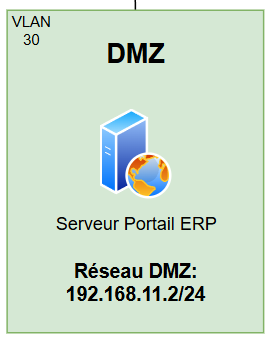
\includegraphics[width=0.2\textwidth]{contents/img/dmz.png}
\end{center}

\noindent Cette zone constitue une barrière de sécurité essentielle entre le réseau externe non fiable et le LAN interne. Aucune communication directe entre Internet et le LAN n’est autorisée ; tous les flux transitent par le pare-feu \textbf{NGFW}, qui applique des règles de filtrage restrictives.

\newpage

\noindent Sur le site de Springfield, l’isolation est également appliquée :
\begin{itemize}
    \item un VLAN Laboratoire pour les machines de test et de développement ;
    \item un VLAN dédié aux imprimantes ;
    
    \vspace{0.5cm}
    \begin{center}
        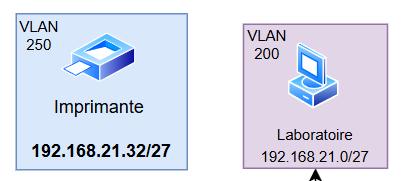
\includegraphics[width=0.4\textwidth]{contents/img/vlan_labo.png}
    \end{center}

    \item une salle serveurs distincte hébergeant un RODC, des serveurs Linux et un NAS local.

    \vspace{0.5cm}
    \begin{center}
        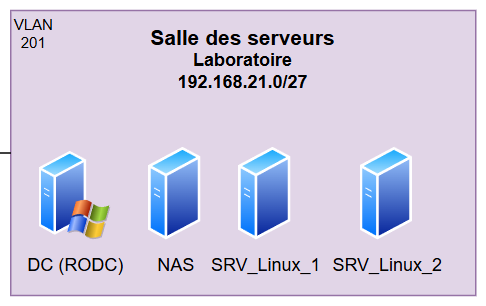
\includegraphics[width=0.4\textwidth]{contents/img/serveurs_labo.png}
    \end{center}

\end{itemize}

\noindent La présence d’un \textbf{RODC (Read Only Domain Controller)} renforce la sécurité du site distant en empêchant toute modification de l’Active Directory depuis ce site, tout en permettant l’authentification locale en cas de coupure du lien WAN.

\noindent Enfin, une \textbf{zone hors ligne Air Gap} est physiquement isolée du réseau. 

    \vspace{0.5cm}
    \begin{center}
        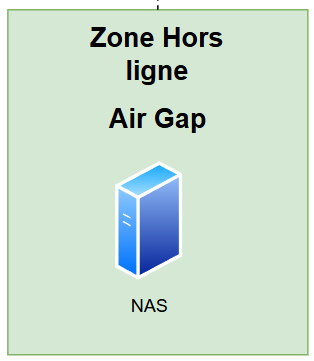
\includegraphics[width=0.2\textwidth]{contents/img/airgap.png}
    \end{center}

\noindent Elle constitue une dernière ligne de défense contre les attaques avancées, notamment les ransomwares, en garantissant l’existence d’une sauvegarde inaccessible depuis le réseau.

\newpage

\subsection*{Optimisation}
\phantomsection
\addcontentsline{toc}{subsection}{Optimisation}

La \textbf{segmentation} mise en place contribue également à l’optimisation globale du système d’information, tant sur le plan des performances que de l’exploitation.

La séparation des flux par VLAN permet :
\begin{itemize}
    \item de réduire les domaines de broadcast et donc la charge réseau ;
    \item d’améliorer la qualité de service pour les applications critiques (ERP, AD, DNS) ;
    \item de faciliter la mise en place de règles de priorisation et de contrôle des flux.
\end{itemize}

\vspace{0.5cm}

\noindent Les \textbf{flux inter-VLAN} sont centralisés et contrôlés au niveau du pare-feu NGFW, ce qui offre une visibilité complète sur les communications internes et externes. Cette centralisation simplifie également l’analyse des incidents et la supervision de la sécurité.

\vspace{0.5cm}

\noindent L’utilisation d’un \textbf{tunnel VPN site-à-site} permet d’optimiser les échanges entre Atlantis et Springfield en assurant une interconnexion transparente et sécurisée. Les utilisateurs du site distant accèdent aux ressources du site principal comme s’ils étaient sur le même réseau logique, sans exposer les services internes à Internet.

\vspace{0.5cm}

\noindent La présence d’un \textbf{proxy Zabbix} à Springfield limite les échanges de supervision sur le lien WAN. Les données sont collectées localement puis synchronisées avec le serveur central, réduisant ainsi la consommation de bande passante et garantissant la continuité de la supervision même en cas de coupure temporaire.
\vspace{0.5cm}

\noindent \textbf{L’architecture virtualisée} des serveurs critiques (ERP, AD, supervision, sauvegarde) permet une meilleure utilisation des ressources matérielles, une plus grande flexibilité lors des opérations de maintenance et une reprise plus rapide en cas d’incident, en cohérence avec les objectifs de PCA et PRA.

\subsection*{L’adressage}
\phantomsection
\addcontentsline{toc}{subsection}{L’adressage}

Le plan \textbf{d’adressage IP} a été conçu de manière hiérarchique, lisible et évolutive, afin de faciliter l’administration, le dépannage et l’extension future de l’infrastructure.

\noindent Chaque VLAN est associé à un sous-réseau distinct en \texttt{/27} pour les réseaux utilisateurs, garantissant un nombre d’adresses suffisant tout en limitant la surface d’attaque et les diffusions inutiles. Les réseaux serveurs utilisent des plages plus larges lorsque nécessaire, comme le réseau interne principal en \texttt{/24}.

\newpage

\noindent Sur le site d’Atlantis :
\begin{itemize}
    \item les VLAN métiers disposent chacun de leur propre sous-réseau ;
    \item le réseau serveurs internes est regroupé sur un sous-réseau dédié ;
    \item la DMZ utilise un sous-réseau distinct (\texttt{192.168.11.0/24}), clairement identifié comme zone exposée.
\end{itemize}

\vspace{0.5cm}

\noindent Sur le site de Springfield :
\begin{itemize}
    \item le VLAN Laboratoire et le VLAN Imprimantes sont séparés ;
    \item la salle serveurs dispose de son propre sous-réseau ;
    \item la zone Air Gap ne dispose pas d’adressage routable permanent.
\end{itemize}

\vspace{0.5cm}

\noindent Ce découpage permet :
\begin{itemize}
    \item une identification immédiate de l’origine d’un flux réseau ;
    \item une application précise des règles de filtrage et de sécurité ;
    \item une évolutivité maîtrisée en cas d’ajout de nouveaux services ou sites.
\end{itemize}

\vspace{0.5cm}

\noindent L’ensemble du plan d’adressage s’inscrit dans une logique de cohérence globale, facilitant la supervision, la journalisation et les audits de sécurité, tout en renforçant la maîtrise opérationnelle du système d’information de XANADU.

\newpage

\section*{Interconnexion et Mobilité}
\addcontentsline{toc}{section}{Interconnexion et Mobilité}

\subsection*{VPN Site-à-Site}
\phantomsection
\addcontentsline{toc}{subsection}{VPN Site-à-Site}

Afin d’assurer une communication sécurisée et continue entre les sites \textbf{Atlantis} et \textbf{Springfield}, une architecture VPN a été mise en place. 

    \vspace{0.5cm}
    \begin{center}
        \begin{minipage}{0.2\textwidth}
            \centering
            \textbf{Atlantis}
        \end{minipage}
        \hfill
        \begin{minipage}{0.5\textwidth}
            \centering
            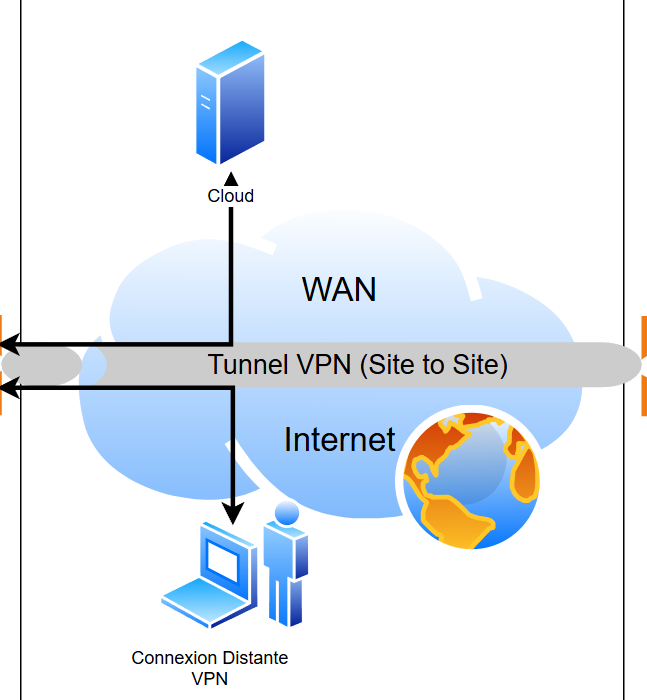
\includegraphics[width=\textwidth]{contents/img/vpn_sitetosite.png}
        \end{minipage}
        \hfill
        \begin{minipage}{0.2\textwidth}
            \centering
            \textbf{Springfield}
        \end{minipage}
    \end{center}


\vspace{0.5cm}

\noindent Le VPN \textit{site-to-site} permet de relier de manière permanente les réseaux locaux des deux sites à travers Internet de façon chiffrée. 

\noindent Ce choix garantit :
\begin{itemize}
    \item \textbf{Une interconnexion sécurisée} entre les infrastructures distantes : le tunnel chiffré protège les flux de données contre toute interception extérieure.
    \item \textbf{L’accès aux ressources internes} (serveurs, partages, sauvegardes) comme si les sites étaient sur un même réseau local, facilitant le travail collaboratif entre les deux entités.
    \item \textbf{La continuité d’activité} en cas de besoin d’accès aux données hébergées sur l’autre site, assurant une haute disponibilité du Système d'Information (SI).
    \item \textbf{Le support du PCA/PRA}, notamment pour les restaurations et les échanges de sauvegardes, permettant de respecter les objectifs de \textit{Recovery Time Objective} (RTO) et \textit{Recovery Point Objective} (RPO).
\end{itemize}

\newpage

\noindent Ce VPN est essentiel pour la réplication, la gestion centralisée et la cohérence du système d’information. Il assure une interconnexion permanente et transparente, indispensable à la survie de l'activité en cas de sinistre sur l'un des sites.

\subsection*{VPN Client}
\phantomsection
\addcontentsline{toc}{subsection}{VPN Client}

Le VPN \textit{client-to-site} permet aux utilisateurs ou administrateurs autorisés de se connecter à distance au réseau interne de manière sécurisée. 

    \vspace{0.5cm}
    \begin{center}
        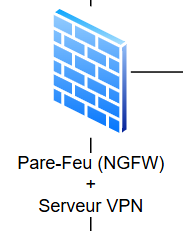
\includegraphics[width=0.2\textwidth]{contents/img/vpn_client.png}
    \end{center}

\noindent Ce mécanisme complète l'architecture réseau en offrant une flexibilité essentielle.

\noindent Il est utilisé pour :
\begin{itemize}
    \item \textbf{Le télétravail sécurisé :} les collaborateurs accèdent à leurs outils habituels via une connexion authentifiée et protégée.
    \item \textbf{Les interventions d’administration à distance :} les techniciens peuvent maintenir les serveurs critiques (ERP, ADDS) sans être physiquement sur place.
    \item \textbf{L’accès aux ressources internes sans exposition directe sur Internet :} cela réduit la surface d'attaque en évitant d'ouvrir des ports sensibles sur le web.
\end{itemize}

\noindent Ce mécanisme renforce la sécurité tout en conservant de la flexibilité opérationnelle, garantissant ainsi que la mobilité des utilisateurs ne compromette pas l'intégrité du réseau de l'entreprise.

\newpage

\section*{Haute Disponibilité et Services Critiques}
\phantomsection
\addcontentsline{toc}{section}{Haute Disponibilité et Services Critiques}

\subsection*{Redondance du Contrôleur de Domaine (DC)}
\phantomsection
\addcontentsline{toc}{subsection}{Redondance du DC}

La mise en place d’une redondance des contrôleurs de domaine (Domain Controllers – DC) sur le site principal d’Atlantis constitue un élément fondamental de la stratégie de haute disponibilité et de sécurité du système d’information de XANADU.  
Cette redondance permet de prévenir et résoudre les problèmes matériels et d'assurer une disponibilité maximale du SI.  

\vspace{0.5cm}
\begin{center}
    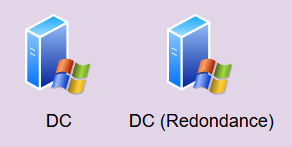
\includegraphics[width=0.4\textwidth]{contents/img/domaine_controller.png}
\end{center}

\vspace{0.5cm}

\noindent \textbf{L’Active Directory (AD)} représente le cœur du système d’information, assurant notamment :
\begin{itemize}
    \item l’authentification et l’autorisation des utilisateurs,
    \item la gestion des droits d’accès aux ressources,
    \item l’application des stratégies de sécurité (GPO),
    \item l’accès aux services essentiels (ERP, VPN, fichiers, messagerie).
\end{itemize}

\noindent La compromission ou l’indisponibilité d’un DC peut paralyser totalement le système d’information. La redondance ne constitue donc pas seulement un mécanisme de disponibilité, mais également une mesure de sécurité active.

\subsubsection*{Continuité de l’authentification}
\noindent Sans redondance, une panne matérielle, une saturation ou une maintenance du DC principal peut entraîner :
\begin{itemize}
    \item l’impossibilité pour les utilisateurs de se connecter,
    \item l’échec de l’application des GPO,
    \item le blocage de l’accès aux services critiques,
    \item une perte de capacité d’action des équipes IT en situation de crise.
\end{itemize}

\noindent La redondance permet aux postes et serveurs de disposer de plusieurs DC disponibles.

\noindent Même en cas de dégradation, d’isolement temporaire ou de maintenance, l’authen-tification reste fonctionnelle, garantissant la continuité de l’activité et la capacité de répondre aux incidents de sécurité.

\subsubsection*{Résilience face aux attaques ciblant l’Active Directory}
\noindent Les DC sont des cibles privilégiées pour les attaquants via :
\begin{itemize}
    \item les attaques sur Kerberos,
    \item l’exploitation du DNS intégré à l’AD,
    \item des attaques par déni de service (DoS),
    \item des ransomwares ou corruptions logiques.
\end{itemize}
\noindent La redondance répartit la charge et les rôles, rendant une attaque isolée inefficace et augmentant la difficulté pour un attaquant de neutraliser l’ensemble du SI.

\subsubsection*{Sécurisation des mises à jour et des évolutions AD}
\noindent Les mises à jour du système ou de l’AD, ainsi que les modifications de GPO ou du schéma AD, peuvent introduire des risques. La redondance permet :
\begin{itemize}
    \item une application progressive des mises à jour,
    \item des tests et validations avant généralisation,
    \item une isolation rapide d’un DC défaillant,
    \item une restauration ciblée sans interruption globale du service.
\end{itemize}

\subsubsection*{Protection contre la corruption logique de l’AD}
\noindent Les ransomwares ou scripts malveillants peuvent altérer les GPO, désactiver ou créer des comptes. La redondance permet de détecter les incohérences, restaurer l’état de l’AD et améliorer le rollback grâce aux sauvegardes.

\subsubsection*{Sécurisation du service DNS}
\noindent Le DNS intégré à l’AD est critique pour la résolution des flux internes. La redondance assure une résolution DNS redondante, augmentant la tolérance aux pannes et limitant l’impact des attaques par saturation ou empoisonnement.

\subsubsection*{Réduction du risque humain}
\noindent Les erreurs d’administration sont une cause majeure d’incidents. La redondance permet de restaurer un DC sans interrompre la disponibilité globale, assurant la continuité opérationnelle.

\newpage

\subsubsection*{Respect des contraintes métiers}
\noindent Cette architecture permet de respecter les exigences de XANADU :
\begin{itemize}
    \item un RTO de 4 heures pour les services critiques,
    \item l’absence de point de défaillance unique,
    \item une meilleure résilience face aux attaques,
    \item une journalisation continue même en cas d’incident.
\end{itemize}

\vspace{0.5cm}

\subsection*{RODC sur le site de Springfield}
\phantomsection
\addcontentsline{toc}{subsection}{RODC à Springfield}

Le site distant de Springfield héberge un laboratoire, avec des machines Linux, et dépend d’un lien MPLS.

\vspace{0.5cm}
\begin{center}
    
\includegraphics[width=0.1\textwidth]{contents/img/rodc_labo.png}
\end{center}

\noindent La mise en place d’un \textbf{RODC (Read Only Domain Controller)} offre plusieurs avantages :
\begin{itemize}
    \item sécurité renforcée, car les mots de passe sensibles ne sont pas stockés localement,
    \item confinement des attaques à l’échelle locale, sans possibilité de modifier l’AD,
    \item continuité de l’activité, les utilisateurs pouvant s’authentifier localement en cas de coupure du MPLS,
    \item amélioration des performances grâce à l’authentification locale réduisant la latence et les échanges réseau.
\end{itemize}

\vspace{0.5cm}

\noindent Le RODC offre donc une solution comprenant de la disponibilité et de la sécurité pour le site distant de Springfield tout en protégeant le système d’information de XANADU et en permettant un maintien de l’activité du laboratoire même en cas de coupure du lien MPLS entre les deux sites.

\newpage

\subsection*{Supervision}
\phantomsection
\addcontentsline{toc}{subsection}{Supervision}

La supervision informatique englobe l’ensemble des outils, techniques et processus permettant de surveiller en continu le matériel, les logiciels et le réseau.  

\vspace{0.5cm}
\begin{center}
    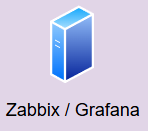
\includegraphics[width=0.2\textwidth]{contents/img/supervision.png}
\end{center}

\subsubsection*{Outils de supervision}
\noindent La solution pour XANADU repose sur :
\begin{itemize}
    \item \textbf{Zabbix} : serveur central, proxy pour sites distants, agents sur serveurs Windows/Linux, collecte et analyse des métriques,
    \item \textbf{SNMP} : supervision des équipements réseau et état du matériel,
    \item \textbf{ICMP} : vérification de la disponibilité et de la latence des liens réseau,
    \item \textbf{Scripts personnalisés} : surveillance spécifique (sauvegardes, ERP, détection de ransomware),
    \item \textbf{Grafana (optionnel)} : visualisation des tableaux de bord et tendances historiques.
\end{itemize}

\subsubsection*{Méthodologie de collecte}
\noindent Les agents Zabbix installés sur les serveurs Windows (AD, DNS, DHCP) et Linux (ERP, laboratoire) collectent CPU, RAM, stockage, services actifs et logs critiques. Les scripts personnalisés assurent la supervision des sauvegardes et la détection des comportements anormaux.  

\noindent La collecte s’effectue en mode :
\begin{itemize}
    \item actif pour les tests ICMP et certaines métriques,
    \item passif pour la majorité des agents, interrogés à la demande par le serveur central.
\end{itemize}

\subsubsection*{Architecture de supervision}
\noindent L’architecture comprend :
\begin{itemize}
    \item un serveur Zabbix sur VM à Atlantis avec base PostgreSQL,
    \item un proxy Zabbix à Springfield pour collecter localement les données et synchroniser lors de la restauration du lien MPLS,
    \item des agents Zabbix sur tous les serveurs critiques, NAS et équipements réseau.
\end{itemize}

\vspace{0.5cm}
\begin{center}
\begin{verbatim}
                +------------------+
                |  Zabbix Server   |  <-- Base PostgreSQL
                |  Atlantis (VM)   |
                +--------+---------+
                         ^
        ICMP/SNMP/Agent | Synchronisation
                         |
                 +-------+--------+
                 | Zabbix Proxy   |  Springfield (VM)
                 | Collecte locale|
                 +-------+--------+
                         ^
         Agents / SNMP / Scripts locaux
                         |
        +----------------+----------------+
        |                |                |
   Serveurs Linux     NAS / Switch     Imprimantes
   Labo Springfield
\end{verbatim}
\end{center}

\subsubsection*{Seuils et alertes}
\noindent Des seuils critiques sont définis pour chaque élément supervisé, déclenchant :
\begin{itemize}
    \item alertes d’avertissement : email à l’équipe IT et aux administrateurs,
    \item alertes critiques : email et message Teams avec escalade temporelle (0–30 min : équipe interne, 30–120 min : CESITECH),
    \item journalisation complète pour audit et traçabilité.
\end{itemize}

\subsubsection*{Conclusion}
\noindent L’architecture de supervision repose sur un serveur central et un proxy distant, utilisant agents, SNMP, ICMP et scripts personnalisés. Elle permet une détection proactive des incidents, une haute disponibilité des services critiques, un respect des SLA et RTO/RPO, tout en restant extensible pour de nouveaux sites ou équipements. Le serveur et le proxy (avec PostgreSQL) peuvent être déployés dans des containers Docker pour plus de résilience et flexibilité.

\newpage

\section*{Sécurité Avancée}
\addcontentsline{toc}{section}{Sécurité Avancée}

\subsection*{DMZ (Zone Démilitarisée)}
\phantomsection
\addcontentsline{toc}{subsection}{DMZ (Zone Démilitarisée)}

Dans le cadre de ce projet, la mise en place d’une \textbf{zone démilitarisée (DMZ – \textit{Demilitarized Zone})} répond à un objectif fondamental de sécurisation de l’architecture réseau.
Une DMZ est une zone intermédiaire située entre un réseau externe, tel qu’Internet, considéré comme non fiable, et le réseau interne de l’entreprise, qui héberge les ressources critiques du système d’information.

\vspace{0.5cm}
\begin{center}
    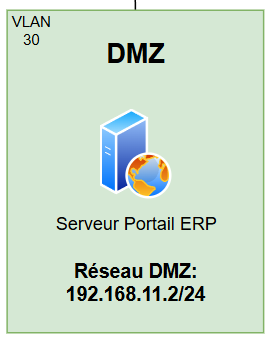
\includegraphics[width=0.2\textwidth]{contents/img/dmz.png}
\end{center}

\noindent Le rôle principal de la DMZ est de permettre l’exposition contrôlée de services accessibles depuis l’extérieur, tout en évitant une exposition directe du réseau interne. Elle agit ainsi comme une zone tampon, limitant les risques d’intrusion et de propagation d’attaques vers les infrastructures sensibles.

\noindent Dans l’architecture retenue, la DMZ a été spécifiquement conçue pour héberger le serveur \textbf{Portail ERP}, un service applicatif nécessitant un accès distant pour les utilisateurs externes. Ce positionnement permet de concilier accessibilité du service, performance et exigences de sécurité, en isolant ce serveur du réseau interne.

\subsubsection*{Enjeux de sécurité et séparation des zones de confiance}

\noindent L’un des principaux enjeux de cette architecture est la protection du réseau interne face aux risques induits par l’exposition de services sur Internet. Tout service accessible depuis l’extérieur constitue un point d’entrée potentiel pour des attaques telles que :
\begin{itemize}
    \item les scans de ports,
    \item l’exploitation de vulnérabilités applicatives,
    \item les attaques automatisées ou par force brute,
    \item les tentatives d’intrusion ciblées.
\end{itemize}

\noindent Placer le serveur Portail ERP directement au sein du réseau local interne (LAN) aurait exposé l’ensemble du système d’information à ces menaces. Une compromission de ce serveur aurait alors pu entraîner un accès direct aux ressources internes, augmentant considérablement l’impact de l’attaque.

\noindent La mise en place d’une DMZ permet au contraire de cloisonner ce service dans une zone de confiance intermédiaire. En cas de compromission du serveur ERP, l’attaquant resterait confiné à la DMZ et ne pourrait accéder au réseau interne qu’au travers de règles de sécurité strictement contrôlées par le pare-feu. Ce principe de cloisonnement constitue une mesure essentielle de défense en profondeur.

\subsubsection*{Rôle du pare-feu pfSense dans la sécurisation de la DMZ}

\noindent Le pare-feu \textbf{pfSense} joue un rôle central dans la sécurisation de l’architecture réseau. Il constitue le point de contrôle unique entre les différentes zones de sécurité :
\begin{itemize}
    \item Internet,
    \item la DMZ,
    \item le réseau interne (LAN).
\end{itemize}

\noindent pfSense assure la segmentation logique du réseau, le filtrage des flux entrants et sortants, ainsi que la gestion fine des règles d’accès entre les zones. Chaque zone bénéficie de politiques de sécurité distinctes, adaptées à son niveau de confiance.

\noindent Le pare-feu permet également la journalisation détaillée des connexions, offrant une visibilité complète sur les flux transitant par la DMZ. Cette fonctionnalité facilite la supervision, l’analyse des événements de sécurité et la détection d’activités suspectes ou anormales.

\subsubsection*{Mise en œuvre technique et segmentation réseau}

\noindent Sur le plan technique, la DMZ est implémentée à l’aide d’un \textbf{VLAN dédié}, le \textbf{VLAN 30}, associé au réseau \textbf{192.168.11.0/24}.  
Cette segmentation logique permet d’isoler efficacement le trafic de la DMZ du reste du réseau, tout en conservant une architecture souple, évolutive et facilement administrable.

\noindent Le serveur Portail ERP est configuré avec une adresse IP fixe (\textbf{192.168.11.2}), ce qui facilite :
\begin{itemize}
    \item la mise en place des règles de filtrage sur le pare-feu,
    \item les redirections de ports depuis Internet,
    \item le contrôle précis des flux autorisés.
\end{itemize}

\noindent Cette organisation améliore la lisibilité de l’infrastructure réseau et permet une gestion fine et maîtrisée des communications entre les différentes zones.

\subsubsection*{Politique de filtrage et contrôle des flux}

\noindent La politique de sécurité appliquée repose sur le principe du \textbf{moindre privilège}. Ce principe consiste à n’autoriser que les flux strictement nécessaires au fonctionnement des services, tout autre trafic étant bloqué par défaut.
Les connexions en provenance d’Internet sont limitées aux seuls services exposés par le serveur ERP hébergé dans la DMZ. Les communications entre la DMZ et le réseau interne sont volontairement restreintes aux échanges indispensables au fonctionnement applicatif.  
Aucune connexion directe entre Internet et le réseau interne n’est autorisée.

\vspace{0.5cm}


\begin{center}
\textbf{Tableau 3 – Synthèse des flux autorisés}
\end{center}

\vspace{0.5cm}

\begin{center}
\begin{tabular}{|l|l|l|c|}
\hline
\textbf{Source} & \textbf{Destination} & \textbf{Type de flux} & \textbf{Autorisation} \\
\hline
Internet & Serveur ERP (DMZ) & Accès applicatif (ports définis) & Autorisé \\
Internet & LAN interne & Tous & Interdit \\
DMZ & LAN interne & Flux applicatifs nécessaires & Restreint \\
LAN interne & DMZ & Administration / Supervision & Autorisé \\
\hline
\end{tabular}
\end{center}

\vspace{0.5cm}

\noindent Ce contrôle strict des flux permet de limiter les risques de propagation d’une attaque, de réduire la surface d’exposition du système d’information et de garantir que chaque communication répond à un besoin fonctionnel clairement identifié.

\subsubsection*{Choix d’une DMZ dédiée et minimaliste}

\noindent Le choix a été fait de concevoir une DMZ volontairement \textbf{minimaliste}, hébergeant uniquement le serveur Portail ERP. Cette approche permet :
\begin{itemize}
    \item de réduire significativement la surface d’attaque,
    \item de simplifier la gestion des règles de sécurité,
    \item d’améliorer la maintenabilité et la lisibilité de l’architecture.
\end{itemize}

\noindent La DMZ est ainsi considérée comme une zone fonctionnelle dédiée à un service précis, et non comme une extension du réseau interne. Cette conception s’inscrit pleinement dans les bonnes pratiques de sécurité des systèmes d’information, notamment celles recommandées par l’ANSSI, en matière de cloisonnement des zones de confiance et de défense en profondeur.

\subsubsection*{Conclusion}

\noindent La mise en place de la DMZ constitue un élément clé de l’architecture réseau du projet. Elle permet d’exposer le serveur Portail ERP de manière sécurisée, tout en protégeant efficacement le réseau interne contre les menaces externes.

\noindent Grâce à l’utilisation de pfSense comme pare-feu central, à la segmentation via un VLAN dédié et à une politique de filtrage rigoureuse fondée sur le principe du moindre privilège, l’architecture répond aux exigences de sécurité, de lisibilité et d’évolutivité attendues dans un environnement professionnel.

\newpage

\subsection*{Sauvegarde}
\phantomsection
\addcontentsline{toc}{subsection}{Sauvegarde}

Le plan de sauvegarde mis en place pour XANADU repose sur la règle de sécurité \textbf{3-2-1}, reconnue comme une bonne pratique de référence en cybersécurité et recommandée par l’ANSSI.
L’objectif de ce plan est de garantir les exigences de \textbf{Continuité d’Activité (PCA)} et de \textbf{Reprise après Incident (PRA)}, tout en respectant les contraintes de \textbf{RTO} et de \textbf{RPO} définies par la Direction.

\noindent La sauvegarde constitue un pilier fondamental de la résilience du système d’information. Elle permet de faire face aux incidents matériels, aux erreurs humaines, ainsi qu’aux cyberattaques de type ransomware ou corruption logique des données.

\noindent \textbf{Objectifs de récupération : RTO et RPO}

\noindent Les objectifs de récupération sont définis à partir des besoins métier :

\begin{itemize}
    \item \textbf{RTO (Recovery Time Objective)} : durée maximale acceptable pour restaurer un service ou une donnée après un incident.
    \item \textbf{RPO (Recovery Point Objective)} : perte de données maximale acceptable, exprimée comme l’intervalle de temps entre la dernière sauvegarde valide et l’incident.
\end{itemize}

\vspace{0.5cm}

\begin{center}
\small
    \begin{tabular}{|p{3cm}|p{8cm}|c|c|}
        \hline
        \textbf{Catégorie} & \textbf{Exemples} & \textbf{RTO} & \textbf{RPO} \\
        \hline
        Critiques & Base de données ERP, données Direction / Juridiques & $\leq$ 4h & $\leq$ 4h \\
        Moyennement critiques & Fichiers partagés & $\leq$ 24h & $\leq$ 24h \\
        Peu critiques & Dossiers personnels centralisés & $\leq$ 24h & $\leq$ 24h \\
        \hline
    \end{tabular}
\end{center}

\vspace{0.5cm}

\noindent \textbf{Application de la règle 3-2-1}

\noindent La règle \textbf{3-2-1} garantit une protection optimale des données :

\noindent
\begin{minipage}[t]{0.68\textwidth}
\textbf{Application de la règle 3-2-1}

La règle \textbf{3-2-1} garantit une protection optimale des données :

\begin{itemize}
    \item \textbf{3 copies des données} :
    \begin{itemize}
        \item Serveur de production (salle des serveurs)
        \item NAS interne
        \item Stockage Cloud
    \end{itemize}

    \item \textbf{2 supports de stockage différents} :
    \begin{itemize}
        \item NAS (interne et externe)
        \item Cloud
    \end{itemize}

    \item \textbf{1 copie hors site} :
    \begin{itemize}
        \item Cloud, conformément aux recommandations de l’ANSSI
    \end{itemize}
\end{itemize}
\end{minipage}
\hfill
\begin{minipage}[t]{0.30\textwidth}
\vspace{-1cm}
\centering
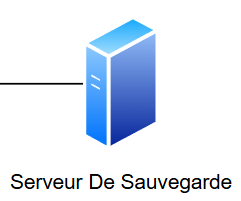
\includegraphics[width=0.6\textwidth]{contents/img/sauvegarde.png}\\[0.3cm]

\includegraphics[width=0.3\textwidth]{contents/img/nas_interne.png}

\includegraphics[width=0.3\textwidth]{contents/img/nas_externe.png}\\[0.3cm]
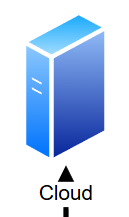
\includegraphics[width=0.3\textwidth]{contents/img/cloud.png}
\end{minipage}


\noindent Le Cloud permet de se prémunir contre les sinistres majeurs tels qu’un incendie, un vol ou une panne totale du site principal, tout en offrant des garanties de disponibilité via des SLA contractuels.

\vspace{0.5cm}

\noindent \textbf{Planification des sauvegardes}

\noindent La planification des sauvegardes est définie selon la criticité des données :

\vspace{0.5cm}

\begin{center}
\small
    \begin{tabular}{|p{2.2cm}|p{2cm}|p{4.5cm}|p{2.5cm}|p{1.8cm}|}
        \hline
        \textbf{Données} & \textbf{Criticité} & \textbf{Fréquence} & \textbf{Rétention} & \textbf{Archivage} \\
        \hline
        ERP / Dossiers partagés & Critiques & Incr./Diff. 4h + complète hebdo & 14j NAS + 3 mois Cloud & 5 ans \\
        Données partagées / Emails & Importantes & Incr. quotidiennes + complète hebdo & 1 mois & 5 à 7 ans \\
        Dossiers personnels & Moins critiques & Incr. quotidiennes + complète hebdo & 7 jours & -- \\
        \hline
    \end{tabular}
\end{center}

\vspace{0.5cm}

\noindent La stratégie repose sur une combinaison de sauvegardes \textbf{complètes}, \textbf{différentielles} et \textbf{incrémentielles}. Les sauvegardes complètes sont réalisées hebdomadairement, de préférence le dimanche soir, afin de limiter l’impact sur l’activité en semaine.
Les sauvegardes différentielles toutes les 4 heures pour les serveurs ADDS et les machines virtuelles ERP permettent de respecter un \textbf{RTO de 4 heures}. Les sauvegardes incrémentielles de la base de données ERP assurent quant à elles le respect du \textbf{RPO de 4 heures}, en capturant rapidement les transactions récentes sans surcharge du système.

\noindent La rétention est organisée sur plusieurs niveaux : une rétention courte sur NAS interne pour les restaurations rapides, une rétention longue via le Cloud pour répondre aux obligations légales, et une conservation hors ligne mensuelle garantissant une capacité de retour arrière étendue.

\vspace{0.5cm}

\noindent \textbf{PCA et PRA}

\noindent Le \textbf{Plan de Reprise d’Activité (PRA)} vise à restaurer les services critiques sous un délai maximal de 4 heures, tandis que les services non critiques doivent être restaurés sous 24 heures.
Les sauvegardes complètes hebdomadaires constituent la base de restauration, complétées par des sauvegardes incrémentielles et différentielles pour limiter la perte de données.

\vspace{0.5cm}

\noindent Le \textbf{Plan de Continuité d’Activité (PCA)} est renforcé par l’utilisation d’un Cloud souverain respectant des SLA contractuels, la priorisation des données critiques lors des restaurations, ainsi que par une architecture haute disponibilité (cluster de serveurs, stockage RAID 10).

\noindent La disponibilité de matériel de rechange (disques, switchs, composants critiques) permet également de réduire significativement les temps d’indisponibilité.

\vspace{0.5cm}

\noindent \textbf{Solution logicielle recommandée : Veeam Backup \& Replication}

\noindent La solution \textbf{Veeam Backup \& Replication} est recommandée pour la mise en œuvre de cette stratégie.
Veeam repose sur des sauvegardes au niveau image (\textit{Image-level Backup}), permettant la restauration complète d’une machine virtuelle, la restauration granulaire de fichiers ou d’objets applicatifs, ainsi que le démarrage instantané d’une VM (\textit{Instant VM Recovery}).

\noindent La solution supporte nativement la règle 3-2-1, la réplication vers des NAS et le Cloud, et intègre des fonctionnalités avancées telles que \textbf{SureBackup} et le \textbf{Change Block Tracking (CBT)}, garantissant le respect des RPO critiques fixés par la Direction.

\subsection*{Air Gap (Zone Hors ligne)}
\phantomsection
\addcontentsline{toc}{subsection}{Air Gap (Zone Hors ligne)}

\noindent Une zone \textbf{Air Gap} est mise en place via un NAS externe isolé et non accessible en permanence depuis le réseau.

\vspace{0.5cm}
\begin{center}
    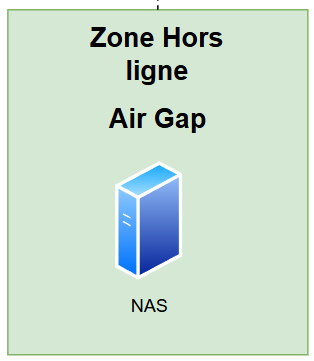
\includegraphics[width=0.3\textwidth]{contents/img/airgap.png}
\end{center}

\vspace{0.5cm}

\noindent Cette approche constitue la dernière ligne de défense face aux attaques de type ransomware ou aux compromissions avancées.

\noindent Les caractéristiques de cette zone Air Gap sont les suivantes :
\begin{itemize}
    \item Données sauvegardées hors ligne et hors portée d’une compromission réseau
    \item Conservation d’une sauvegarde complète mensuelle des données critiques
    \item Capacité de restauration fiable en cas d’infection persistante ou d’erreur humaine ancienne
\end{itemize}

\vspace{0.5cm}

\noindent Les sauvegardes stockées dans cette zone sont conservées pendant une durée d’un an, garantissant un point de restauration sûr, indépendant du réseau et du Cloud.
L’Air Gap assure ainsi l’existence d’un point de reprise absolument fiable, même dans les scénarios d’attaque les plus graves, et renforce significativement la résilience globale du système d’information de XANADU.

\newpage

\section*{Surcoûts entraînés}
\phantomsection
\addcontentsline{toc}{section}{Surcoûts entraînés}

\subsubsection*{Analyse des surcoûts et justification des choix techniques}

Dans le cadre du projet XANADU, plusieurs choix techniques ont été réalisés au-delà des exigences minimales du cahier des charges initial. Ces choix engendrent des surcoûts financiers, volontairement assumés afin d’augmenter significativement le niveau de sécurité, de résilience et de pérennité du système d’information.

\noindent Les décisions prises s’appuient sur les recommandations de l’ANSSI, sur les bonnes pratiques observées en PME, ainsi que sur une estimation réaliste des coûts basée sur les tarifs publics des éditeurs de solutions professionnelles et sur des retours d’expérience du monde professionnel.

\subsubsection*{Solution antivirus professionnelle centralisée}

Le premier surcoût notable concerne la mise en place d’une solution antivirus professionnelle centralisée, en remplacement d’un antivirus natif ou grand public. Bien que Windows Defender intégré aux systèmes Windows offre une protection de base satisfaisante, il présente des limites importantes dans un environnement professionnel, notamment en matière de visibilité globale, de corrélation des incidents et de réponse centralisée.

\noindent Les solutions antivirus grand public ont été écartées, car elles ne sont pas conçues pour une intégration avec un Active Directory et ne permettent pas une administration homogène du parc informatique. Le choix d’une solution professionnelle centralisée, telle que Microsoft Defender for Endpoint ou une solution équivalente, permet une supervision globale des postes et serveurs, une détection comportementale avancée des ransomwares et une intégration native avec l’annuaire Active Directory.

\noindent Les coûts associés à ce type de solution sont estimés entre 5 et 8 euros par utilisateur et par mois. Pour une entreprise de 60 utilisateurs, cela représente un surcoût annuel compris entre \textbf{3 600 et 5 760 euros}, auquel s’ajoute un coût indirect lié à l’administration et à la supervision. Ce surcoût est justifié par le niveau de protection apporté et par les recommandations de l’ANSSI.

\subsubsection*{Interconnexion WAN via une infrastructure cloud}

Un second surcoût est lié à l’utilisation d’une infrastructure cloud comme point d’interconnexion WAN entre les sites d’Atlantis et de Springfield. Une solution MPLS privée aurait présenté un coût élevé (entre 300 et 600 euros par mois), une faible flexibilité et une dépendance forte à l’opérateur télécom.

\noindent À l’inverse, une interconnexion reposant uniquement sur Internet public aurait réduit les coûts, mais au détriment de la résilience et de la qualité de service. Le recours au cloud, associé à des tunnels VPN chiffrés, permet de bénéficier d’une haute disponibilité native, d’une grande flexibilité et d’un déploiement rapide.

\newpage

\noindent Les coûts d’une passerelle VPN cloud sont estimés entre \textbf{50 et 150 euros par mois}, soit environ \textbf{600 à 1 800 euros par an}. Cette solution respecte les recommandations de l’ANSSI, sous réserve d’un chiffrement strict des flux.

\subsubsection*{Pare-feux de nouvelle génération}

La sécurisation périmétrique du système d’information repose sur l’utilisation de pare-feux de nouvelle génération (NGFW), engendrant un surcoût par rapport à un filtrage réseau basique. Les solutions minimales offrent une visibilité limitée et peu de capacités de détection.

\noindent Les NGFW permettent une inspection applicative des flux, une journalisation détaillée, la détection d’intrusions et une gestion centralisée des tunnels VPN. Les coûts estimés pour des équipements adaptés aux PME sont compris entre \textbf{1 500 et 3 000 euros à l’achat}, auxquels s’ajoutent des licences annuelles de sécurité estimées entre \textbf{500 et 1 000 euros par an}. Ce choix s’inscrit dans une logique de défense en profondeur recommandée par l’ANSSI.

\subsubsection*{Architecture VPN hybride}

La mise en place de plusieurs types de VPN constitue également un surcoût. Le VPN site-à-site entre Atlantis et Springfield garantit la confidentialité des échanges inter-sites, tandis que le VPN client-à-site sécurise les accès distants des utilisateurs en mobilité ou en télétravail.

\noindent Une solution unique aurait été moins coûteuse, mais moins adaptée aux usages. Le choix d’une architecture VPN hybride (IPsec et VPN client) entraîne un surcoût estimé entre \textbf{300 et 800 euros par an}, justifié par une meilleure séparation des flux et un niveau de sécurité renforcé.

\subsubsection*{Redondance de l’Active Directory}

La redondance de l’Active Directory constitue un autre surcoût significatif. Bien que non imposée par le cahier des charges, elle répond à la criticité de ce composant, souvent ciblé par les attaques.

\noindent La mise en place d’un contrôleur de domaine secondaire sur le site principal et d’un RODC sur le site distant engendre un surcoût lié aux ressources matérielles ou virtuelles. Ces coûts sont estimés entre \textbf{500 et 1 000 euros par serveur}, soit \textbf{1 000 à 2 000 euros} pour l’ensemble, hors coûts d’administration. Ce choix améliore significativement la résilience et la sécurité du SI, conformément aux recommandations de l’ANSSI.

\subsubsection*{Politique de sauvegarde renforcée}

La politique de sauvegarde mise en œuvre dépasse les exigences minimales en intégrant la règle du 3-2-1 et un stockage isolé de type \textit{air gap}. Une solution plus simple aurait été moins coûteuse, mais vulnérable aux ransomwares.

\noindent Cette architecture implique l’acquisition d’un NAS professionnel, estimé entre \textbf{1 000 et 2 000 euros}, ainsi que des licences de sauvegarde professionnelles comprises entre \textbf{500 et 1 000 euros par an}. Ce surcoût garantit une capacité de reprise fiable en cas d’incident majeur.

\subsubsection*{Conclusion}

Les surcoûts observés dans le projet XANADU ne constituent pas des dépenses superflues, mais des investissements stratégiques visant à renforcer la sécurité, la disponibilité et la résilience du système d’information.

\noindent Sur la base des estimations présentées, le coût initial d’investissement (équipements et serveurs) est estimé entre \textbf{3 500 et 7 000 euros}.  
Les coûts récurrents annuels (licences, services cloud, sécurité et sauvegardes) sont quant à eux estimés entre \textbf{5 800 et 11 200 euros par an}.

\noindent Chaque choix technique a été réalisé après comparaison de plusieurs alternatives, en retenant la solution offrant le meilleur compromis entre coût, sécurité et exploitabilité, dans le respect des bonnes pratiques et des recommandations de l’ANSSI.

\newpage

\section*{Conclusion}
\addcontentsline{toc}{section}{Conclusion}

Le projet XANADU avait pour objectif principal la modernisation, la sécurisation et la pérennisation du système d’information de l’entreprise dans un contexte de croissance et de multi-sites. À travers l’ouverture du site de Springfield et le déménagement vers la technopole Atlantis, il était essentiel de concevoir une architecture capable de répondre aux enjeux actuels de cybersécurité, de continuité d’activité et de mobilité des utilisateurs.

\noindent L’architecture proposée repose sur une segmentation réseau stricte par VLAN, une interconnexion sécurisée des sites via des tunnels VPN chiffrés, ainsi qu’une séparation claire des zones de confiance (LAN, DMZ, Air Gap). Cette approche permet de limiter la surface d’attaque, de réduire les déplacements latéraux en cas de compromission et de garantir une maîtrise fine des flux réseau, conformément aux principes de défense en profondeur recommandés par l’ANSSI.

\noindent La mise en œuvre de services critiques hautement disponibles, tels que l’Active Directory redondé, le RODC sur le site distant, la supervision centralisée via Zabbix et une politique de sauvegarde avancée basée sur la règle du 3-2-1, assure une forte résilience du système d’information. Ces choix techniques permettent de respecter les objectifs de PCA et PRA définis par la Direction, notamment un RTO de 4 heures pour les services critiques et une capacité de reprise fiable face aux incidents majeurs, y compris les attaques par ransomware.

\noindent La sécurité a été pensée comme un élément transversal de l’architecture : pare-feux de nouvelle génération, antivirus professionnel centralisé, DMZ dédiée au portail ERP, VPN hybrides et sauvegardes hors ligne constituent un ensemble cohérent visant à protéger les données, les utilisateurs et les services tout en conservant une flexibilité opérationnelle adaptée aux besoins métiers.

\noindent Ces choix impliquent des surcoûts maîtrisés, assumés comme des investissements stratégiques. Le coût initial d’investissement est estimé entre \textbf{3 500 et 7 000 euros}, tandis que les coûts récurrents annuels liés aux licences, aux services cloud, à la sécurité et aux sauvegardes sont évalués entre \textbf{5 800 et 11 200 euros par an}. Ces montants restent cohérents avec les pratiques observées en PME et sont justifiés par le niveau de sécurité, de disponibilité et de fiabilité obtenu.

\noindent En conclusion, l’architecture proposée pour XANADU constitue une solution robuste, évolutive et sécurisée, capable d’accompagner durablement l’entreprise dans son développement. Elle offre un équilibre pertinent entre contraintes budgétaires, exigences métiers et recommandations institutionnelles, tout en posant des bases solides pour l’évolution future du système d’information, notamment en cas d’ouverture de nouveaux sites ou d’intégration de nouveaux services.


